% This is not a step-by-step instruction or diary to your work.
% Instead, you should describe your technical approach and solution, describe architecture, components, etc.
% Think software engineering...
% Perhaps use a few useful uml-diagrams or illustrate the system architecture.
% Keep in mind that the purpose of the implementation section is to describe your implementation to solve the problems from 1.3.
 
% This section can have a lot of subsections, example:
% 4.1 System architecture / System arkitektur
% 4.2 System components / System komponenter
% 4.3 ...

TODO

\begin{figure}[h]
    \centering
    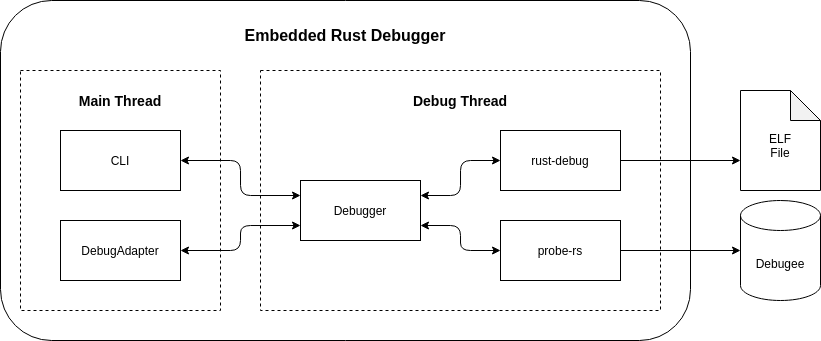
\includegraphics[width=1.0\textwidth]{debugger_structure.png}
    \label{fig:EDBStruct}
\end{figure}

\subsection{Debug Library}
\import{implementation/}{debug_library.tex}

\subsection{Debugger}
\import{implementation/}{debugger.tex}

\subsection{Command Line Interface}
\import{implementation/}{cli.tex}

\subsection{Debug Adapter}
\import{implementation/}{debug_adapter.tex}

\subsection{VSCode Extension}
\import{implementation/}{vscode_extension.tex}

